\documentclass[tikz, border=15pt]{standalone}
\usepackage{amsmath}
\usetikzlibrary{shapes.geometric, arrows.meta, positioning, fit, backgrounds}

\begin{document}

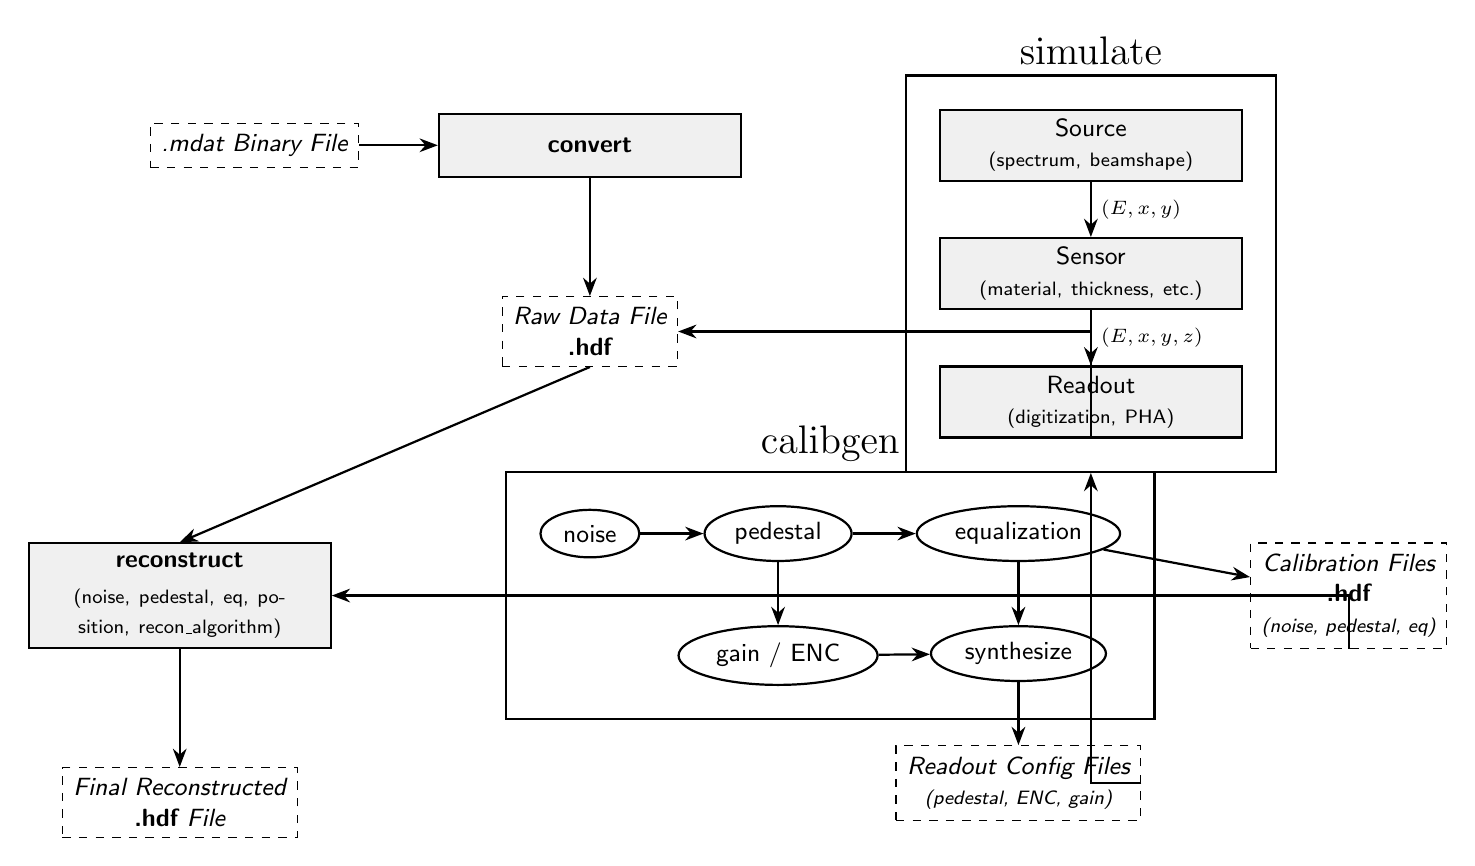
\begin{tikzpicture}[
    node distance=0.7cm and 1.2cm,
    % Stili dei nodi
    proc/.style={rectangle, draw=black, thick, fill=gray!12, text width=3.6cm, minimum height=0.8cm, align=center, font=\small\sffamily},
    subcmd/.style={ellipse, draw=black, thick, fill=white, inner sep=3pt, font=\small\sffamily, align=center},
    io/.style={rectangle, draw=black, dashed, fill=white, inner sep=4pt, font=\small\sffamily\itshape, align=center},
    group/.style={rectangle, draw=black, thick, inner sep=12pt, font=\small\sffamily\bfseries},
    arrow/.style={-Stealth, thick}
]

    % ==================== INPUT / SOURCING ====================
    \node [io] (mdat) {.mdat Binary File};
    \node [proc, right=1.0cm of mdat] (convert) {\textbf{convert}};

    % ==================== SIMULATE CONTAINER ====================
    \node [proc, right=2.5cm of convert] (source) {Source \\ \scriptsize (spectrum, beamshape)};
    \node [proc, below=of source] (sensor) {Sensor \\ \scriptsize (material, thickness, etc.)};
    \node [proc, below=of sensor] (readout) {Readout \\ \scriptsize (digitization, PHA)};

    \node[group, fit=(source) (sensor) (readout), label={above:\Large simulate}] (sim_box) {};

    % Connessioni interne simulate
    \draw [arrow] (source) -- node[right, font=\scriptsize\sffamily] {$(E, x, y)$} (sensor);
    \draw [arrow] (sensor) -- node[right, font=\scriptsize\sffamily] {$(E, x, y, z)$} (readout);

    % ==================== DATA HDF5 FILE ====================
    % Nodalizziamo il file hdf generato da convert o simulate
    \node [io, below=1.5cm of convert] (hdf_data) {Raw Data File \\ \textbf{.hdf}};

    % Frecce che creano il file Raw .hdf
    \draw [arrow] (convert) -- (hdf_data);
    \draw [arrow] (readout.south) |- (hdf_data.east);
    \draw [arrow] (mdat) -- (convert);


    % ==================== CALIBGEN CONTAINER ====================
    \node [subcmd, below=1.8cm of hdf_data] (cal_noise) {noise};
    \node [subcmd, right=0.8cm of cal_noise] (cal_pedestal) {pedestal};
    \node [subcmd, right=0.8cm of cal_pedestal] (cal_eq) {equalization};
    
    \node [subcmd, below=0.8cm of cal_pedestal] (cal_gain) {gain / ENC};
    \node [subcmd, below=0.8cm of cal_eq] (cal_synth) {synthesize};

    \node[group, fit=(cal_noise) (cal_pedestal) (cal_eq) (cal_gain) (cal_synth), label={above:\Large calibgen}] (calib_box) {};

    % Flusso interno calibgen
    \draw [arrow] (cal_noise) -- (cal_pedestal);
    \draw [arrow] (cal_pedestal) -- (cal_eq);
    \draw [arrow] (cal_pedestal) -- (cal_gain);
    \draw [arrow] (cal_eq) -- (cal_synth);
    \draw [arrow] (cal_gain) -- (cal_synth);

    % File prodotti da calibgen
    \node [io, right=1.2cm of calib_box] (calib_files) {Calibration Files \\ \textbf{.hdf} \\ \scriptsize (noise, pedestal, eq)};
    \node [io, below=0.8cm of cal_synth] (sim_config_files) {Readout Config Files \\ \scriptsize (pedestal, ENC, gain)};

    % Frecce di output da calibgen
    \draw [arrow] (cal_eq) -- (calib_files);
    \draw [arrow] (cal_synth) -- (sim_config_files);

    % Loopback di calibgen verso il readout di simulate
    \draw [arrow] (sim_config_files.east) -| (sim_box.south);


    % ==================== RECONSTRUCT CONTAINER ====================
    \node [proc, left=2.2cm of calib_box] (recon) {\textbf{reconstruct} \\[2pt] \scriptsize (noise, pedestal, eq, position, recon\_algorithm)};

    \node [io, below=1.5cm of recon] (final_hdf) {Final Reconstructed \\ \textbf{.hdf} File};

    % Connessioni in ingresso a Reconstruct
    \draw [arrow] (hdf_data.south) -- (recon.north);
    \draw [arrow] (calib_files.south) |- (recon.east);
    
    % Connessione in uscita da Reconstruct
    \draw [arrow] (recon) -- (final_hdf);

\end{tikzpicture}

\end{document}